\section{Introduction}

Knowing whether an event of interest will occur is crucial. However, in many situations, knowing when
it will occur can be even more informative. In this context, a statistical methodology known as survival
analysis arises. The elapsed time until the occurrence of an event of interest is referred to as the
survival time \cite{aalen2008survival}. For example, in a study concerned with loan default among credit
union members, the survival time may be defined as the time until a member defaults on a loan. Survival
analysis is therefore concerned with modeling the distribution of this time and investigating factors that
may influence its occurrence. Thus, the objective of this chapter is to present the fundamental
concepts underlying survival analysis.


\section{Censoring}

The main characteristic that distinguishes survival analysis from other areas of statistics is the presence
of censored data. For example, consider a study in which credit union members are followed over time to
investigate the occurrence of loan default. In this context, two situations may happen. Some members may
default during the follow-up period, whereas others may not experience the event before the end of the
study. In the latter case, censoring occurs because the survival time of these individuals is not fully
observed; it is only known that the event will occur after a certain point in time.

Censoring can occur in three different forms. The example described above can be regarded as right
censoring. Right censoring occurs when the event takes place after a certain time, but its exact occurrence
time is unknown. Another type is left censoring, which occurs when the event has taken place before a
certain time. In the context of loan default, an example of left censoring would be a member who was
already in default at the beginning of the study, while the exact time at which the default occurred is
unknown. Finally, interval censoring occurs when the event takes place within a given time interval, but
its exact occurrence time is unknown. Given the loan default example, interval censoring could arise if
members were evaluated periodically and default was detected only during these assessments, without
knowledge of the exact time at which it occurred. Figure \ref{fig:censoring_system} illustrates each type
of censoring.

\begin{figure}[htb]
    \centering
    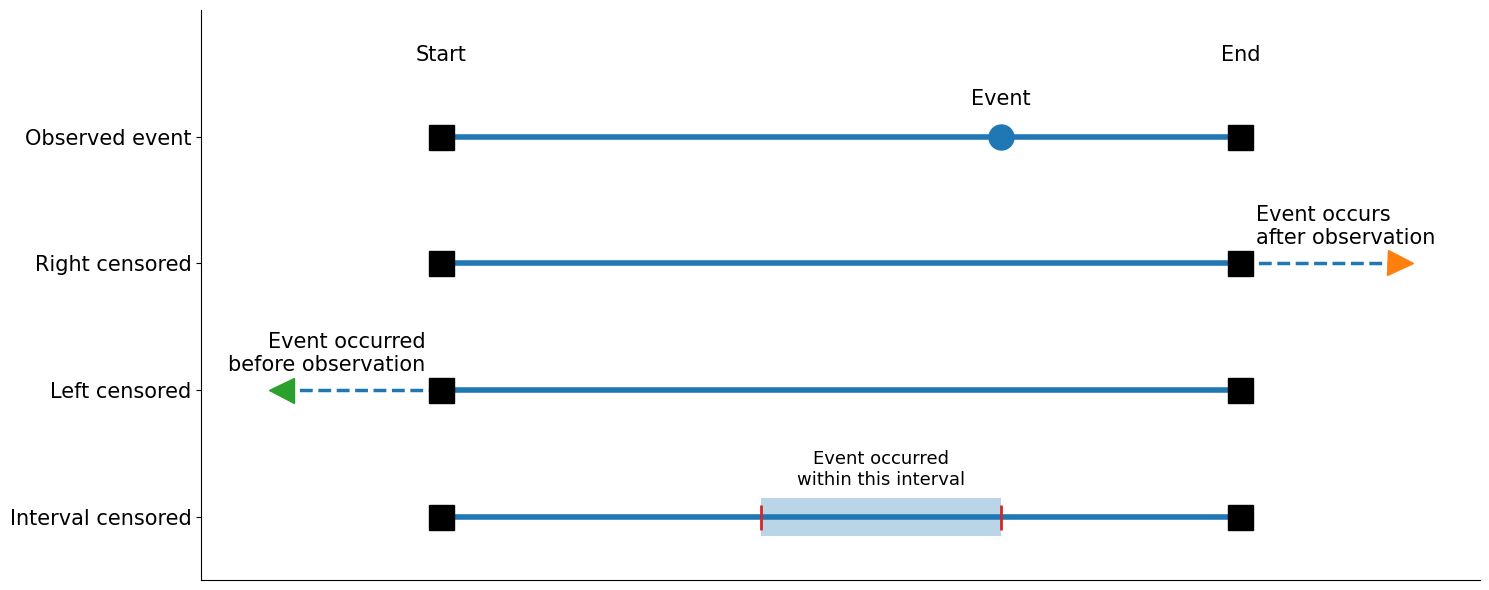
\includegraphics[width=0.8\textwidth]{images/figure_censore_representation.png}
	\caption{Illustration of observed events and censoring types in survival analysis: observed event, right censoring, left censoring, and interval censoring.}
    \label{fig:censoring_system}
\end{figure}

Formally, let \(T\) denote the survival time and let \(l\) and \(u\) denote the lower and upper bounds of
the censoring interval, respectively. Under interval censoring, it is only known that \(l < T \leq u\),
where both \(l\) and \(u\) are finite. Notice that left and right censoring can be viewed as special cases
of interval censoring. Hence, left censoring corresponds to the interval \((-\infty, u]\), whereas
right censoring corresponds to the interval \((l, \infty)\).

The methods presented in this work consider only right censoring, since it is the most common type
encountered in practice. Thus, to represent survival data, let \(T^*\) be a random variable representing
the time to failure, i.e., the time until the occurrence of the event of interest, and let \(U\) be a
random variable representing the time to a censoring event. The observed time is \(T = \min(T^*, U)\) and a
censoring indicator \(\delta = I[T^* \leq U]\). That is, \(\delta\) takes the value 0 or 1 according to
whether \(T\) is an observed failure time or a censored time \cite{moore2016applied}. Hence, throughout
this work, survival data will be represented by the triplet \(\{(\mathbf{x}_i, t_i, \delta_i)\}_{i=1}^{n}\),
where \(\mathbf{x}_i \in \mathbb{R}^{p}\) denotes the vector of covariates, \(t_i\) the observed time, and
\(\delta_i\) an indicator variable associated with the \(i\)-th individual. The sample size is denoted by
\(n\), and \(p\) denotes the number of covariates.

Therefore, survival data are generally composed of both complete and incomplete observations
\cite{aalen2008survival}. As a result, survival analysis methods seek to incorporate censored observations
into their methodology. Given the definition of censoring presented in this section, the next section
introduces the definitions of the survival function and hazard rate, as well as some relationships
between these functions.

\section{Survival and hazard rate functions}

Survival analysis is concerned with the study of the time until the occurrence of an event of interest. A survival distribution can be characterized through several equivalent functions, among which the survival function and the hazard rate function are fundamental \cite{moore2016applied}. The survival function describes the probability that the event has not occurred by a given time $t$. Formally, let $T$ denote the nonnegative random variable representing the survival time. The survival function is defined as
\begin{equation}
\label{eq:surv_function}
S(t) = P(T > t), \qquad t \geq 0.
\end{equation}

Thus, $S(t)$ represents the probability that an individual survives beyond time $t$, or,
equivalently, that the event of interest has not occurred by that time. The survival
function is a non-increasing function satisfying $S(0)=1$ and $\lim_{t\to\infty} S(t) \geq 0$.

In the usual setting, the survival function decreases as $t$ increases, reflecting the
accumulation of events over time. However, it need not converge to zero. In particular,
if $\lim_{t\to\infty} S(t) = 0$, the corresponding distribution is said to be proper.
Conversely, when $\lim_{t\to\infty} S(t) > 0$, the distribution is said to be
improper. The latter case is of particular relevance in cure-rate models, where
the positive limiting value of the survival function can be interpreted as the
probability of an individual belonging to a cured fraction. This distinction will be
discussed in greater detail in the next section.

The hazard rate function, denoted by $h(t)$, characterizes the instantaneous risk of experiencing the event of interest, conditional on survival up to time $t$. More precisely, assuming that $T$ is an absolutely continuous random variable with probability density function $f(t)$, the hazard rate at time $t$ is defined as
\begin{equation}
\label{eq:hazard_function}
h(t)
=
\lim_{\Delta t \to 0}
\frac{1}{\Delta t}
P\left(t \leq T < t+\Delta t \mid T \geq t\right).
\end{equation}

Thus, for a sufficiently small time interval $\Delta t$, the quantity
\[
h(t)\Delta t
\]
provides a first-order approximation to the conditional probability of experiencing the
event during the interval $[t,t+\Delta t)$, given that the individual has survived up
to time $t$. It is important to note that the hazard rate itself is not a probability
and, consequently, is not restricted to the interval $[0,1]$.

Under the assumption of absolute continuity, the hazard rate can be expressed in terms
of the probability density function and the survival function as
\begin{equation}
\label{eq:hazard_density_survival}
h(t)
=
\frac{f(t)}{S(t)}\text{.}
\end{equation}
Conversely, the survival function can be recovered from the hazard rate through the
cumulative hazard function, defined as
\begin{equation}
\label{eq:cumulative_hazard}
H(t)
=
\int_0^t h(u)\,du.
\end{equation}
Consequently,
\begin{equation}
\label{eq:survival_hazard}
S(t)
=
\exp\left\{-H(t)\right\}
=
\exp\left\{-\int_0^t h(u)\,du\right\}.
\end{equation}

Equation \eqref{eq:survival_hazard} establishes the fundamental relationship between the hazard
rate and the survival function. In particular, the survival function is determined
by the cumulative hazard over time. Consequently, different hazard profiles may lead to
substantially different survival patterns, even when they are defined on the same time
scale.

\begin{figure}[htb]
    \centering
    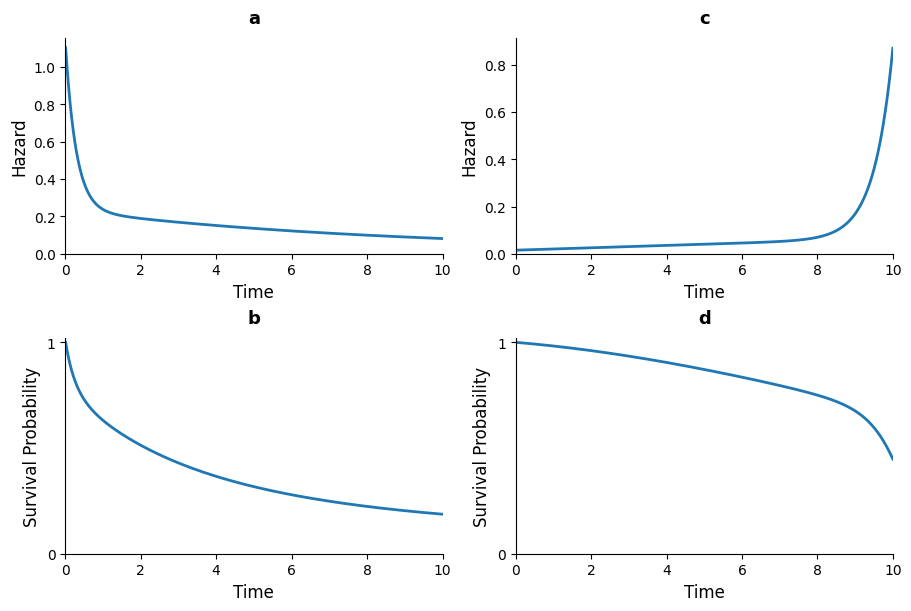
\includegraphics[width=0.8\textwidth]{images/relation_between_harzard_and_survival_function.png}
	\caption{Illustration of observed events and censoring types in survival analysis: observed event, right censoring, left censoring, and interval censoring.}
    \label{fig:relation_survival_hazard}
\end{figure}

Figure \ref{fig:relation_survival_hazard} illustrates this relationship. In panels (a)
and (b), the hazard rate is relatively high at early times, resulting in a more pronounced
decline in the corresponding survival function. Such a pattern may arise, for example,
in populations characterized by a high risk of death shortly after entering the study.
In contrast, panels (c) and (d) illustrate a hazard with a lower initial risk,
leading to a slower decline in the corresponding survival function. These examples emphasize that
the shape of the survival function is directly determined by the evolution of the
hazard rate over time.

Although the survival and hazard rate functions provide two fundamental ways of
characterizing a survival distribution, other distributional functions are also useful,
particularly when deriving likelihoods and establishing relationships among different
representations of the survival distribution. Among these, the cumulative distribution
function and the probability density function are of particular importance.

The cumulative distribution function (CDF) of the survival time $T$ is defined by
\begin{equation}
\label{eq:cdf}
F(t) = P(T \leq t),
\end{equation}
and, for a nonnegative random variable, is related to the survival function through
\begin{equation}
\label{eq:cdf_survival}
F(t) = 1-S(t).
\end{equation}

When $T$ is absolutely continuous, its probability density function (PDF) is given by
the derivative of the CDF,
\begin{equation}
\label{eq:pdf}
f(t) = \frac{d}{dt}F(t)
     = -\frac{d}{dt}S(t).
\end{equation}
Consequently, the principal functions associated with an absolutely continuous survival
distribution are connected through
\[
f(t) = h(t)S(t),
\]
which follows directly from the definition of the hazard rate.

These relationships provide equivalent representations of the same underlying survival
distribution. In particular, knowledge of any one of the functions, under the appropriate
regularity conditions, allows the others to be obtained. The relationships among these
functions will be used throughout the subsequent development of the survival and cure-rate
models considered in this work.

\subsection{Likelihood for censored survival times}

In the absence of censoring, suppose that the survival times $T_1^*,\ldots,T_n^*$
are independent and identically distributed with probability density function
$f(t;\boldsymbol{\theta})$ and survival function $S(t;\boldsymbol{\theta})$, where
$\boldsymbol{\theta}$ denotes the vector of model parameters. The likelihood function
based on the complete survival times is then given by
\begin{equation}
\label{eq:complete_likelihood}
L(\boldsymbol{\theta})
=
\prod_{i=1}^{n} f(t_i^*;\boldsymbol{\theta}).
\end{equation}

In practice, however, survival times are frequently subject to right censoring. As defined
previously, let $T^*$ denote the time to failure and $U$ the censoring time. The observed
time and censoring indicator are given by $T=\min(T^*,U) \text{ and } \delta=I[T^*\leq U]$,
respectively. Thus, $\delta=1$ indicates that the event of interest was observed, whereas
$\delta=0$ indicates that the observation was right-censored.

Accordingly, the observed survival data considered throughout this work are represented
by the triplet $\left\{(\boldsymbol{x}_i,t_i,\delta_i)\right\}_{i=1}^{n}$,
where $\boldsymbol{x}_i\in\mathbb{R}^{p}$ denotes the vector of covariates for the
$i$th individual, $t_i$ is the observed time, and $\delta_i$ is the corresponding event
indicator.

For an individual with $\delta_i=1$, the event is observed at time $t_i$, and the
likelihood contribution is given by the density $f(t_i;\boldsymbol{\theta})$. In
contrast, when $\delta_i=0$, the event has not occurred by time $t_i$, and the available
information is that $T_i^*>t_i$. Consequently, the likelihood contribution is given by
the survival probability $S(t_i;\boldsymbol{\theta})$. These two cases can be combined
into the single expression
\begin{equation}
\label{eq:individual_likelihood}
L_i(\boldsymbol{\theta})
=
f(t_i;\boldsymbol{\theta})^{\delta_i}
S(t_i;\boldsymbol{\theta})^{1-\delta_i}.
\end{equation}

Assuming independence among individuals, the likelihood function based on the observed survival data is therefore
\begin{equation}
\label{eq:observed_likelihood}
L(\boldsymbol{\theta})
=
\prod_{i=1}^{n}
f(t_i;\boldsymbol{\theta})^{\delta_i}
S(t_i;\boldsymbol{\theta})^{1-\delta_i}.
\end{equation}

Using the relationship $f(t;\boldsymbol{\theta})=h(t;\boldsymbol{\theta})S(t;\boldsymbol{\theta})$, the likelihood can equivalently be expressed in terms of the hazard rate as
\begin{equation}
\label{eq:hazard_likelihood}
L(\boldsymbol{\theta})
=
\prod_{i=1}^{n}
h(t_i;\boldsymbol{\theta})^{\delta_i}
S(t_i;\boldsymbol{\theta}).
\end{equation}

This formulation is fundamental in survival analysis because it accounts simultaneously
for observed failures and right-censored observations. It will also provide the basis
for the likelihood formulations considered later for the long-term survival and
cure-rate models developed in this work.

In conventional survival models, it is typically assumed that every individual is
eventually susceptible to the event, implying that $\lim_{t\to\infty}S(t)=0$. However,
this assumption may be inappropriate in settings where a subset of individuals is
considered effectively immune to the event of interest. In such cases, the survival
function may converge to a positive limiting value, $\lim_{t\to\infty}S(t)=\pi>0$, where
$\pi$ represents the asymptotic probability of remaining event-free.
This behavior is characteristic of cure-rate models and provides a natural framework
for explicitly modeling a cured fraction within the population. The distinction between
these two settings is central to the development of cure-rate models and will be
considered in the following section.

\section{Long-term survival models}

In some survival studies, a non-negligible proportion of individuals may never experience
the event of interest, even when followed for an arbitrarily long period of time. Such
individuals are commonly referred to as cured or immune with respect to
the event under consideration \cite{maller1996survival}. The presence of such individuals gives
rise to the class of models commonly referred to as long-term survival models or
cure-rate models.

This setting differs fundamentally from that of conventional survival models, which
generally assume that every individual is susceptible to the event of interest and that
the event will eventually occur with probability one. Under this assumption, the
survival function satisfies
\begin{equation}
\lim_{t\rightarrow\infty} S(t)=0.
\end{equation}
In contrast, when a proportion of the population is not susceptible to the event, the
population survival function may converge to a positive value,
\begin{equation}
\lim_{t\rightarrow\infty} S(t)=\pi,
\qquad 0<\pi<1,
\end{equation}
where $\pi$ represents the long-term survival probability, commonly interpreted as the
population cure fraction.

The formulation of long-term survival models considered in this work follows the
extension proposed by \citeonline{rodrigues2009unification}.
In this extension, the occurrence of the event of interest is represented through a
collection of competing causes. Let $N$ be a random variable denoting the number of
competing causes related to the occurrence of the event of interest, with probability
distribution
\begin{equation}
\label{eq:N_distribution}
p_n=P(N=n), \qquad n=0,1,2,\ldots.
\end{equation}

Conditional on $N=n$, let $Z_1,\ldots,Z_n$ denote the latent times to the event
associated with these causes. Assume that these random variables are independent and
identically distributed, with proper survival function $S(t)$ that does not depend on
$N$. In order to include individuals who are not susceptible to the event, the event
time is defined as the minimum among the latent times,
\begin{equation}
\label{eq:latent_event_time}
T=\min\{Z_1,\ldots,Z_N\},
\end{equation}
with $P\left(Z_{0} = \infty\right) = 1$, which leads to a proportion $p_0$ of the population
not susceptible to the event occurrence.

Given the previous definitions, let $\{a_n\}$ be a real-valued sequence and
$s\in[0,1]$. The generating function \cite{feller1971introduction}, denoted by
$A(s)$, of the sequence $\{a_n\}$ is given by
\begin{equation}
\label{eq:generating_function}
A(s)=a_0+a_1s+a_2s^2+\ldots.
\end{equation}

The survival function of the random variable $T$ is then obtained as
\begin{eqnarray}
\label{eq:long_term_survival}
S_p(t) &=& P(N=0) + P(Z_1>t,Z_2>t,\ldots,Z_N>t,N\geq1) \nonumber \\
&=& P(N=0) + \sum_{n=1}^{\infty}P(N=n)
P(Z_1>t,Z_2>t,\ldots,Z_n>t) \nonumber \\
&=& p_0+\sum_{n=1}^{\infty}p_n\{S(t)\}^n \nonumber \\
&=& A\left(S(t)\right),
\end{eqnarray}
where $A(\cdot)$ is the generating function associated with the probability
mass function $\{p_n\}$, as defined in Equation \eqref{eq:generating_function},
and $S(t)$ is a proper survival function. Since $\lim_{t\rightarrow0}S(t)=1$ and
$\lim_{t\rightarrow\infty}S(t)=0$, it follows that $\lim_{t\rightarrow\infty}S_p(t) = A(0) = P(N=0) = p_0$.

Thus, when $p_0>0$, the long-term survival function has a positive limiting value,
which can be interpreted as the proportion of individuals in the population who are
not susceptible to the event of interest, i.e., the cure fraction. Consequently,
$S_p(t)$ is an improper survival function. It is a non-increasing function and satisfies
$S_p(0)=1$.

The probability density function and the hazard rate function associated with the long-term
survival function are given, respectively, by
\begin{eqnarray}
f_{p}(t) = f(t)\frac{dA(s)}{ds}|_{s=S(t)}\text{,}
\end{eqnarray}
\begin{eqnarray}
h_{p}(t) = \frac{f_{p}(t)}{S_{p}(t)}=f(t)\frac{\frac{dA(s)}{ds}|_{s=S(t)}}{S_{p}(t)}.
\end{eqnarray}


\begin{table}[htb]
    \centering
    \caption{Long-term survival, density, hazard, and cure fraction for the different
    distributions considered for the latent number of competing causes $N$.}
    \label{tab:long_term_models}
    \scriptsize
    \renewcommand{\arraystretch}{1.15}
    \setlength{\tabcolsep}{3pt}
    \resizebox{\textwidth}{!}{%
    \begin{tabular}{c|c|c|c|c}
        \hline
        Distribution of $N$
        & $S_p(t)$
        & $f_p(t)$
        & $h_p(t)$
        & $p_0$ \\
        \hline

        Bernoulli$(\theta)$
        &
        $1-\theta+\theta S(t)$
        &
        $\theta f(t)$
        &
        $\dfrac{\theta f(t)}
        {1-\theta+\theta S(t)}$
        &
        $1-\theta$
        \\[2mm]

        $\text{Binomial}\left(K,\theta^* = \frac{\theta}{1 + \theta}\right)$
        &
        $\left[1-\theta^*+\theta^*S(t)\right]^K$
        &
        $K\theta^*f(t)
        \left[1-\theta^*+\theta^*S(t)\right]^{K-1}$
        &
        $\dfrac{K\theta^*f(t)}
        {1-\theta^*+\theta^*S(t)}$
        &
        $(1-\theta^*)^K$
        \\[2mm]

        Negative Binomial$(\alpha,\theta)$
        &
        $\{1+\alpha\theta\left[1-S(t)\right]\}^{-1/\alpha}$
        &
        $\theta f(t)
        \{1+\alpha\theta\left[1-S(t)\right]\}^{-1/\alpha-1}$
        &
        $\dfrac{\theta f(t)}
        {1+\alpha\theta\left[1-S(t)\right]}$
        &
        $(1+\alpha\theta)^{-1/\alpha}$
        \\[2mm]

        Poisson$(\theta)$
        &
        $\exp\{-\theta[1-S(t)]\}$
        &
        $\theta f(t)\exp\{-\theta[1-S(t)]\}$
        &
        $\theta f(t)$
        &
        $e^{-\theta}$
        \\[2mm]

        \hline
    \end{tabular}%
    }
\end{table}

The methods developed in this work consider different distributions for the latent variable
$N$, representing the number of competing causes. Specifically, the Bernoulli, Binomial, Negative
Binomial, and Poisson distributions are considered. The corresponding results are summarized in
Table~\ref{tab:long_term_models}, and their derivations are given below, beginning
with the Bernoulli distribution.

\subsection{Bernoulli distribution}

Let $N$ be a random variable representing the number of latent competing causes
associated with the occurrence of a given event, following a Bernoulli distribution with
parameter $\theta \in (0,1)$, i.e., $N \sim \text{Bernoulli}(\theta)$. Its probability
mass function is given by
\begin{equation}
P(N=n)
=
\theta^{n}(1-\theta)^{1-n},
\qquad n=0,1.
\end{equation}

The generating function of $N$ is given by
\[
A(s)=1-\theta+\theta s,
\]
and, therefore, the long-term survival function is
\begin{equation}
S_p(t)
=
A\left(S(t)\right)
=
1-\theta+\theta S(t).
\end{equation}
This corresponds to the mixture cure model introduced by \cite{berkson1952survival}, one
of the most widely used models for long-term survival data. The model is referred to as
a mixture cure model because the population survival function can be expressed as a
mixture of a cure component and a proper survival function corresponding to the
susceptible population. In this case, the cure fraction is given by
\begin{equation}
p_0
=
\lim_{t\to\infty}S_p(t)
=
1-\theta.
\end{equation}

The probability density and hazard rate functions are given, respectively, by
\begin{equation}
f_p(t)
=
\theta f(t)
\end{equation}
and
\begin{equation}
h_p(t)
=
\frac{\theta f(t)}
{1-\theta+\theta S(t)}.
\end{equation}

\subsection{Binomial distribution}

The Binomial distribution provides a natural extension of the Bernoulli specification by
allowing the number of latent competing causes to take values from $0$ to $K$. Let $N$
be a random variable representing the number of latent competing causes associated with
the occurrence of the event of interest, following a Binomial distribution with
parameters $K$ and $\theta^*\in(0,1)$, i.e.,
\[
N\sim\mathrm{Binomial}\left(K,\theta^* = \frac{\theta}{1 + \theta}\right),
\]
where $K$ is a positive integer. Its probability mass function is given by
\begin{equation}
\label{eq:binomial_pmf}
P(N=n)
=
\binom{K}{n}
\left(\theta^*\right)^n\left(1-\theta^*\right)^{K-n},
\qquad n=0,1,\ldots,K.
\end{equation}

The probability generating function of $N$ is
\begin{equation}
\label{eq:binomial_pgf}
A(s)
=
\left(1-\theta^*+\theta^*s\right)^K.
\end{equation}
Consequently, the corresponding long-term survival function is
\begin{equation}
\label{eq:binomial_survival}
S_p(t)
=
A\left(S(t)\right)
=
\left[1-\theta^*+\theta^*S(t)\right]^K.
\end{equation}

The cure fraction is obtained by taking the limit as $t\rightarrow\infty$,
\begin{equation}
\label{eq:binomial_cure_fraction}
p_0
=
\lim_{t\rightarrow\infty}S_p\left(t\right)
=
\left(1-\theta^*\right)^K.
\end{equation}

Thus, increasing $K$, while keeping $\theta^*$ fixed, decreases the cure fraction, since
a larger number of potential competing causes increases the probability that at least
one cause is present.

Differentiating \eqref{eq:binomial_survival} with respect to $t$, the corresponding
density function is
\begin{equation}
\label{eq:binomial_density}
f_p\left(t\right)
=
K\theta^*f\left(t\right)
\left[1-\theta^*+\theta^*S\left(t\right)\right]^{K-1},
\end{equation}
where $f\left(t\right)=-S'\left(t\right)$ is the density associated with the proper survival function $S(t)$.
Therefore, the corresponding hazard rate function is
\begin{equation}
\label{eq:binomial_hazard}
h_p\left(t\right)
=
\frac{K\theta^*f\left(t\right)}
{1-\theta^*+\theta^*S\left(t\right)}.
\end{equation}


\subsection{Negative Binomial distribution}

A more flexible specification is obtained by assuming that the number of latent competing
causes follows a Negative Binomial distribution. Let $N$ follow a Negative Binomial
distribution with parameters $\alpha$ and $\theta$, where $\theta>0$ and
$\alpha\theta>-1$. Its probability mass function can be written as
\begin{equation}
\label{eq:negative_binomial_pmf}
P\left(N=n\right)
=
\frac{\Gamma\left(\alpha^{-1}+n\right)}
{\Gamma\left(\alpha^{-1}\right)n!}
\left(\frac{\alpha\theta}{1+\alpha\theta}\right)^n
\left(1+\alpha\theta\right)^{-1/\alpha},
\qquad n=0,1,2,\ldots,
\end{equation}
with the corresponding probability generating function
\begin{equation}
\label{eq:negative_binomial_pgf}
A\left(s\right)
=
\left[1+\alpha\theta(1-s)\right]^{-1/\alpha}.
\end{equation}

The long-term survival function is consequently given by
\begin{equation}
\label{eq:negative_binomial_survival}
S_p\left(t\right)
=
\{1+\alpha\theta\left[1-S\left(t\right)\right]\}^{-1/\alpha}.
\end{equation}
Its cure fraction is
\begin{equation}
\label{eq:negative_binomial_cure_fraction}
p_0
=
\lim_{t\rightarrow\infty}S_p\left(t\right)
=
\left(1+\alpha\theta\right)^{-1/\alpha}.
\end{equation}

Under this parametrization, $E\left[N\right]=\theta$ and $\operatorname{Var}\left(N\right)=\theta+\alpha\theta$.
Therefore, the parameter $\alpha$ controls the dispersion of the number of latent
competing causes. For $\alpha>0$, the distribution is overdispersed relative to a
Poisson distribution, whereas $\alpha<0$ corresponds to underdispersion, subject to the
condition $\alpha\theta>-1$.

This parametrization is particularly useful because it provides a continuous connection
among the Binomial, Poisson, and Negative Binomial distributions. Specifically, when $\alpha=-1/K$,
the Negative Binomial distribution reduces to a Binomial distribution with parameters
$K$ and $\theta/K$, provided that $0\leq\theta/K\leq1$. As $\alpha\rightarrow0$, the
distribution converges to a Poisson distribution with parameter $\theta$. For
$\alpha>0$, it corresponds to the usual overdispersed Negative Binomial formulation.

Differentiating \eqref{eq:negative_binomial_survival}, the density function associated
with the long-term survival distribution is
\begin{equation}
\label{eq:negative_binomial_density}
f_p(t)
=
\theta f(t)
\{1+\alpha\theta\left[1-S(t)\right]\}^{-1/\alpha-1},
\end{equation}
and its hazard rate function is
\begin{equation}
\label{eq:negative_binomial_hazard}
h_p(t)
=
\frac{\theta f(t)}
{1+\alpha\theta\left[1-S(t)\right]}.
\end{equation}

The flexibility of this formulation is particularly relevant for long-term survival
modeling, since it encompasses several important cure-rate models as special or limiting
cases. In particular, the choice $\alpha=-1$ corresponds to the Bernoulli case and
consequently recovers the classical mixture cure model, whereas the limit
$\alpha\rightarrow0$ yields the Poisson model and the corresponding promotion-time cure
model.

\subsection{Poisson distribution}

The Poisson distribution is obtained as the limiting case of the Negative Binomial
formulation when $\alpha\rightarrow0$. Let $N$ follow a Poisson distribution with
parameter $\theta>0$, i.e., $N\sim\mathrm{Poisson}(\theta)$.
Its probability mass function is
\begin{equation}
\label{eq:poisson_pmf}
P(N=n)
=
\frac{e^{-\theta}\theta^n}{n!},
\qquad n=0,1,2,\ldots,
\end{equation}
and its probability generating function is $A(s) = \exp\{\theta(s-1)\}$. Therefore, the
corresponding long-term survival function is
\begin{equation}
\label{eq:poisson_survival}
S_p(t)
=
A\left(S(t)\right)
=
\exp\left\{-\theta[1-S\left(t\right)]\right\}
=
\exp\left\{-\theta F\left(t\right)\right\}.
\end{equation}

The cure fraction is given by $p_0 = \lim_{t\rightarrow\infty}S_p(t) = e^{-\theta}$,
the corresponding density function is $f_p\left(t\right) = \theta f\left(t\right) \exp\{-\theta F\left(t\right)\}$,
and the associated hazard rate function is $h_p\left(t\right) = \theta f\left(t\right)$. The Poisson specification is particularly important in long-term survival analysis
because it leads to the promotion-time cure model \cite{yakovlev1996stochastic}.

The Kaplan--Meier estimator (KME) is one of the most widely used nonparametric
methods for estimating the survival function in the presence of right-censored
observations. In the context of long-term survival analysis, the estimated survival
curve can also provide an indication of the presence of a cure fraction when it
approaches a positive plateau at large observed times. Although the Kaplan--Meier
estimator does not, by itself, identify or consistently estimate the cure fraction
without additional assumptions regarding the follow-up period, it provides a useful
nonparametric reference for assessing whether a long-term survival pattern is
supported by the data. In this work, the Kaplan--Meier estimator is used for this
purpose and to assess whether the proposed long-term survival models adequately
capture the observed survival pattern.

\section{Kaplan--Meier estimator}

The Kaplan--Meier estimator (KME) is one of the most widely used nonparametric
methods for estimating the survival function in the presence of right-censored
observations \cite{kaplan1958nonparametric}. Let $\{(t_i,\delta_i)\}_{i=1}^n$
denote the observed survival data, where $t_i$ is the observed time and
$\delta_i$ is the censoring indicator, with $\delta_i=1$ indicating an observed
event and $\delta_i=0$ indicating right censoring. Let
$t_{(1)}<\cdots<t_{(m)}$ denote the distinct observed event times. If $d_j$
individuals experience the event at $t_{(j)}$ and $Y_j$ individuals are at risk
immediately before $t_{(j)}$, the KME is given by
\begin{equation}
\label{eq:kaplan_meier}
\widehat{S}_{KM}(t)
=
\prod_{t_{(j)}\leq t}
\left(1-\frac{d_j}{Y_j}\right).
\end{equation}

The KME is a step function that changes only at observed event times, while
censored observations contribute to the risk set up to their censoring times.
In the context of long-term survival analysis, a survival curve that approaches
a positive plateau at large follow-up times may provide empirical evidence of a
nonzero long-term survivor fraction. However, such a plateau should be
interpreted with caution, as limited follow-up and heavy censoring can also
produce a positive tail.

In this work, the KME is used as a nonparametric reference for assessing the
long-term survival pattern in the data and for evaluating whether the proposed
long-term survival models adequately capture the observed cure fraction.
